\documentclass[11pt]{article}
 \newcommand{\forceindent}{\leavevmode{\parindent=1.5em\indent}}
\usepackage[utf8]{inputenc}
\usepackage{graphicx}
\usepackage{geometry}
 \geometry{
 a4paper,
 left=1in,
 top=0.75in,
 right=1in,
 bottom=0.75in
 }
 
\linespread{1.5}

 
\begin{document}
\rmfamily
 \noindent Suryansh Singh\\ 
Professor Rota\\         
Linear Optimization\\
April 12, 2021 \\ 

\begin{center}
    {\Large The Four Color Problem }
\end{center}

\noindent \underline{Introduction}\\
The four color theorem states that the regions of any simple planar map can be colored with only four colors, in such a way that any two adjacent regions have different colors. The theorem was first proposed by Francis Gauthrie in 1852 when he noticed while coloring a map of England that he only required four colors to do so. He then discussed this observation to his brother, Frederick Gauthrie who later on went on to discuss the observation with Augustus De Morgan, who was his Mathematics Professor at the University College London. De Morgan is the source for the first written reference to the Four Color Theorem where he referred to the theorem to a fellow Mathematician, William R. Hamilton in a letter asking him about whether he had heard about the theorem or not [4]. From there, the theorem spread throughout mathematical circles and became quite famous. Although this theorem sounds rather simple and is quite easy to comprehend, it however was an extremely hard theorem to prove, with the theorem being conclusively proved only in 1976 by Appel and Haken that too with the aid of a computer. It was in fact the first major theorem that was proved through brute forcing scenarios with a computer [3].  Between 1852 and 1976, there were several false proofs as well that were proposed by several mathematicians. One of the most famous of those proofs that turned out to be false was the one proposed by Alfred Bray Kempe which although it initially seemed to prove the four color theorem was eventually proven false by Percy J. Heawood [4]. Eventually after several failed attempts, it was only in 1976 when Appel and Haken were finally able to prove the four color theorem with the help of a powerful computer. Their proof was really lengthy, but essentially could be simplified to as checking 1,936 cases for reducibility [3]. Being the first major theorem proved by using brute forcing scenarios, the proof has also been a major source of controversy with some questioning its validity even today. Several modern day mathematicians believed that the proof should only be proven by people and not by machines and that somehow using a computer invalidates the proof [1]. Regardless of the doubters, the proof is considered valid although there is still work being done on trying to find a proof to the theorem that does not require a computer although such attempts have still been largely unsuccessful and mathematicians to this day have not yet found a proof to the four color theorem that does not involve the use of computers. \\

\noindent \underline{Kempe's Proof}\\
Alfred Bray Kempe was a barrister based in London who was also a student of Arthur Cayley, a renowned mathematician who had published a paper about the four color theorem and the difficulties surrounding proving it. Kempe is most famously known for coming up with his version of a proof to the four color theorem which was eventually found to be in actuality a false proof. Kempe's Proof essentially used mathematical induction in order to prove the 4 color theorem and we shall show that proof below [4]: \\

\noindent Base Step:\\
Any map containing four or less countries or sections or regions can be colored with at most four different colors. Thus proving the base step.\\

\noindent Inductive Step:\\
Assume that any map that contains $n$ countries or sections or regions can be colored with at most four different colors. Then let $M$ be a map that contains $n+1$ countries or sections or regions. Then there should be a country or region or section which we shall call $X$ be present that is adjacent to five or fewer countries or sections or regions. Now if we were to disregard $X$ for a moment, we are left with the map $M$ which has $n$ countries or sections or regions which we know by our assumption can be colored with using at most four different colors. This leaves us with only $X$ uncolored. Now we shall see all the possible cases and examples that could be possible and were also used for Kempe's proof:\\
I) Case 1:\\
\forceindent If $X$ is surrounded by three or less countries or sections or regions, then there clearly will \forceindent be a color available for $X$. \\
II) Case 2:\\
\forceindent If $X$ is surrounded by exactly four countries or sections or regions as shown in the image \forceindent below.\\
\begin{figure}[ht!]
\centering
\IfFileExists{Kempe1.png}{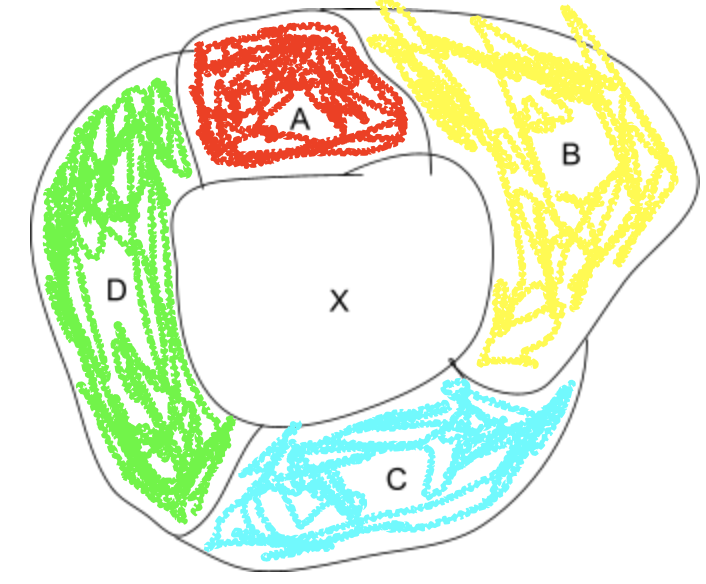
\includegraphics[width=0.2\textwidth]{Kempe1.png}}{No Figure Yet}
\caption{Case 2} 
\end{figure}

A technique that was used by Kempe when he was deriving his proof was using the method we now know as Kempe chains [3]. A Kempe chain is a chain of vertices that are colored with two alternating colors. So keeping that in mind we have two further sub cases for Case 2:\\
\forceindent i) Case 2.1: Suppose $A$ and $C$ belong to two separate Red - Blue Kempe Chains:\\
\forceindent \forceindent For this sub case, if we want to make a color available for $X$, we simply need to take \forceindent \forceindent either one of the Kempe chains and interchange the colors in that chain. So in the \forceindent \forceindent above Figure 1, we can simply interchange the colors for the Red Blue Kempe chain that \forceindent \forceindent contains $C$ in it which would make $C$ also red. As a result, we can use Blue to color in \forceindent \forceindent $X$, thus fulfilling the requirements of our theorem. \\
\forceindent ii) Case 2.2: Suppose $A$ and $C$ belong to the same Red - Blue Kempe Chain:\\
 \forceindent \forceindent For this sub case, if $A$ and $C$ belong to the same Red - Blue Kempe Chain, then \forceindent \forceindent that  would mean that the Red-Blue Kempe Chain between A and C would prevent \forceindent \forceindent the possibility of another continuous Green-Yellow Kempe Chain between $B$ and $D$. \forceindent \forceindent Thus, that means that $B$ and $D$ belong to two separate Green-Yellow Kempe Chains. \forceindent \forceindent So, if we want to make a color available for $X$, we simply need to interchange the   \forceindent \forceindent colors of either the Green-Yellow Kempe Chain containing $B$ or the Green-Yellow  Kempe  \forceindent \forceindent Chain containing $D$. So, for example we could interchange the colors for the Green-Yellow  \forceindent \forceindent Kempe Chain containing $B$ and thus that would meant that $B$ would also be green and  \forceindent \forceindent thus, we can color $X$ with Yellow and thus fulfill the conditions of the four color theorem  \forceindent \forceindent for this particular sub case.\\
 
 III) Case 3:\\
\forceindent If $X$ is surrounded by exactly five countries or sections or regions as shown in the image \forceindent below.\\
\begin{figure}[ht!]
\centering
\IfFileExists{Kempe2.png}{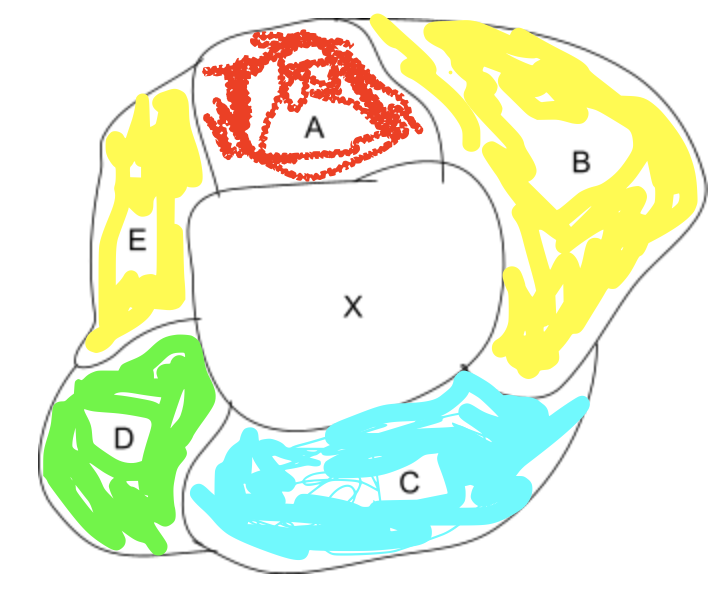
\includegraphics[width=0.2\textwidth]{Kempe2.png}}{No Figure Yet}
\caption{Case 3} 
\end{figure}
 
 There are two further sub cases for Case 3:\\
 \forceindent \forceindent i) Case 3.1: Suppose $A$ and $C$ belong to two separate Red-Blue Kempe Chains:\\
\forceindent \forceindent For this sub case, if we want to make a color available for $X$, we simply need to take \forceindent \forceindent either one of the Kempe chains and interchange the colors in that chain. So in the \forceindent \forceindent above Figure 2, we can simply interchange the colors for the Red-Blue Kempe chain that \forceindent \forceindent contains $C$ in it which would make $C$ also red. As a result, we can use Blue to color in \forceindent \forceindent $X$, thus fulfilling the requirements of our theorem. \\
 \forceindent \forceindent ii) Case 3.2: Suppose Suppose $A$ and $C$ belong to the same Red-Blue Kempe Chain and \forceindent \forceindent $A$ and $D$ as well belong to the same Red-Green Kempe Chain :\\
 \forceindent \forceindent  For this sub case, if $A$ and $C$ belong to the same Red-Blue Kempe Chain and $A$ and \forceindent \forceindent $D$ as well belong to the same Red-Green Kempe Chain, that would mean that $B$ and \forceindent \forceindent $ED$ would not belong to the same Green-Yellow Kempe Chain as the $A$ and $C$ Red-Blue \forceindent \forceindent Kempe Chain and the $A$ and $D$ Red-Green Kempe Chain would effectively prevent a \forceindent \forceindent common Green-Yellow Kempe chain to be present between $B$ and $ED$. Also, since $A$  \forceindent \forceindent and $D$ are part of the same Red-Green Kempe Chain, that means that $E$ and $C$ belong  \forceindent \forceindent to two different Blue-Yellow Kempe Chains. So, if we were to interchange the colors  \forceindent \forceindent of  the Green-Yellow Kempe chain that contains $B$, that would make $B$ Green. Then  \forceindent \forceindent we could interchange the colors of the Blue-Yellow Kempe Chain that contains $E$, thus  \forceindent \forceindent making $E$ Blue. With the interchanging of colors of these two Kempe chains, we have  \forceindent \forceindent managed to free up Yellow that could be used to color $X$ and thus fulfill the requirements  \forceindent \forceindent of our theorem. Hence we prove this sub part as well.\\
 
 \noindent Kempe had similarly like we have shown above proven the inductive part of his proof in a similar manner[4]. However there was a major flaw in his proof that was only discovered ten years later by Percy Heawood.\\
 
 \noindent \underline{Heawood's Counterexample}\\
 After Alfred Kempe had published his proof, he received praise and recognition for his work on the Four Color Theorem. He even was elected a Fellow of the Royal Society even serving as its treasurer at one point as well as being knighted for his work on the Four Color Theorem [3]. However, ten years later, Percy Heawood, a lecturer at Durnham, England submitted a publication which managed to find a major flaw in Alfred Kempe's proof. He was able to find a special case for the sub case 3.2 because of which Kempe's proof would be invalidated. The special case was that the Yellow-Green Kempe chain that contains $B$ might in fact touch the Yellow-Blue Kempe chain that contains $E$, and thus Kempe's method of resolving this as we saw in sub case 3.2 would not work. We can see this in the given example below with an image that fits the conditions of Heawood's special case:
 
 \begin{figure}[ht!]
\centering
\IfFileExists{Haewood.png}{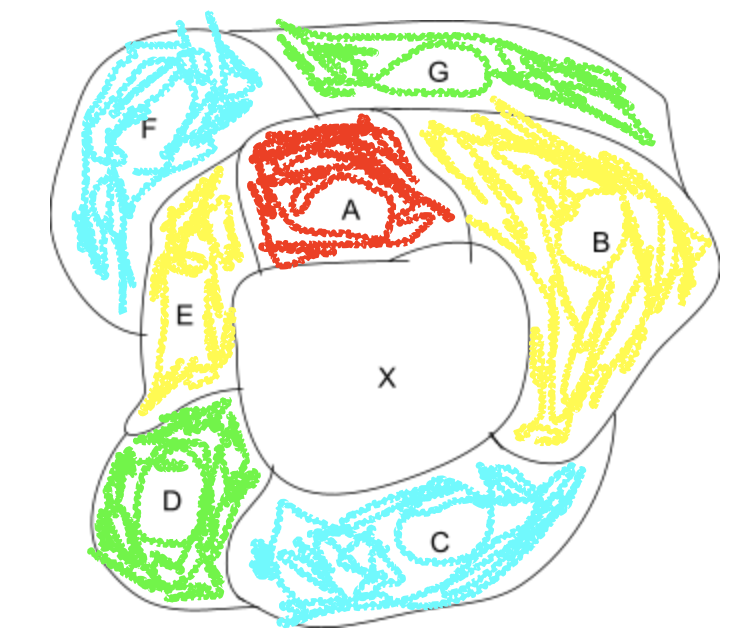
\includegraphics[width=0.15\textwidth]{Haewood.png}}{No Figure Yet}
\caption{ Heawood's Special Case Example} 
\end{figure}
 
 In the above figure, let $F$ be the country or section or region that is a part of the Yellow-Blue Kempe Chain that contains $E$ and touches the Green-Yellow Kempe Chain that contains $B$. Let $G$ be the country or section or region that is a part of the Yellow-Green Kempe Chain that contains $B$ and touches the Green-Yellow Kempe Chain that contains $E$. So, if we were to follow Kempe's proof like he stated for sub case 3.2, then that means we would have to interchange the colors for both the the Yellow-Green Kempe Chain that contains $B$ as well as the Green-Yellow Kempe Chain that contains $E$. However that would result in $F$ becoming yellow as well as $G$ also becoming yellow. But, since $F$ and $G$ touch each other, that means that Kempe's method would not work out as he had planned it to be and thus Kempe's proof was disproved using the above special case. \\
 \forceindent Although, Percy Heawood was the one who found the special case that disproved Kempe's Proof, he was unable to fix the error and be able to prove the theorem himself. Even Kempe, whose proof was disproven tried his best to find a fix to this special case however he was also unsuccessful as well. In fact most mathematicians were unable to find a new way to prove the Four Color Theorem until Appel and Haken were able to prove it using the help of a computer.\\
 
  
 \noindent \underline{Appel and Haken's Proof}\\
 Although, Heawood was unable to prove the Four Color Theorem, he was able to prove the Five Color Theorem which similar to the Four Color Theorem stated that regions of any simple planar map can be colored with only five colors, in such a way that any two adjacent regions have different colors. He was also instrumental in shifting the focus of the proof from the areas of the map to the borders of the map[1]. Mathematicians were also able to by 1900 learnt that a planar graph could be constructed from any map, using the concept of duality [1] which we will describe using the help of an example below:\\
 Example: For the map given in Figure 3, we can represent it as a planar graph by converting the regions into vertices and representing the border regions such that the vertices would be connected by an edge in the graph if they share a border in the map. So for the map given if Figure 3, it would be represented as a planar graph as: \\
 \begin{figure}[ht!]
\centering
\IfFileExists{Duality.png}{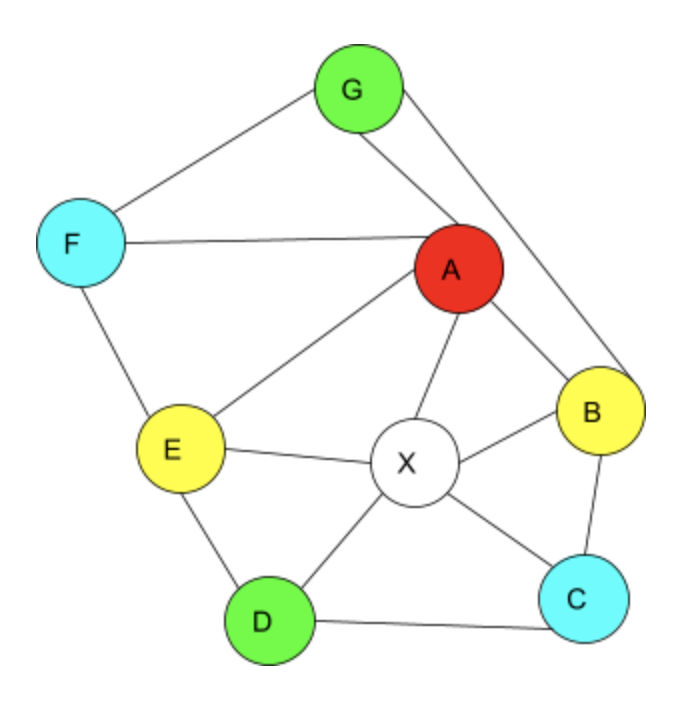
\includegraphics[width=0.2\textwidth]{Duality.png}}{No Figure Yet}
\caption{ Figure 3 represented as a planar graph} 
\end{figure}
 
 Both the original map and the planar graph obey Euler's Formula for networks, which states that $f+v-e = 1$ [1], where $f$ represents regions, $v$ represents vertices, and $e$ represents edges. For our map, we have 8 regions, 14 vertices and 21 edges and thus it obeys the Euler's Formula for networks as $f+v-e = 8 + 14 - 21 = 1$. For our plane we have 8 regions, 8 vertices and 15 edges and thus it also obeys the Euler's Formula for networks as $f+v-e = 8 + 8 - 15 = 1$. The duality relation is symmetric which means that the dual of the dual will be the original graph. Thus we can now incorporate graph theory in the Four Color Theorem.\\
  \forceindent After the conversion of a map to a planar graph, we could now rephrase the four color theorem in Graph Theory such that for any planar graph, the vertices of the graph can be colored with at most four colors such that there are no two adjacent vertices that are of the same color. This helped simplify the theorem and led to mathematicians trying to find the minimal set of special cases which could be represented by graphs and then prove it using Mathematical Induction in a similar fashion that Kempe had done above. Since, the base case was already proved, the induction case was the only part left to be proved and that would have to be done by checking all the possible sub cases that could arise in our proof. This was eventually done by Appel and Haken who finally proved the theorem with the help of a computer. Wolfgang Haken was a German Mathematician who had first raised the question on whether computers could be used to help assist in proving the Four Color Theorem [2]. It was Haken who decided to use a new approach when it came to proving the Four Color Theorem. Instead of collecting reducible configurations by the hundreds and then package them up into an unavoidable set which would be done with the help of the computer, he decided to aim directly for an unavoidable set [2]. This way the computer would not waste time in checking configurations that were unlikely to appear in the eventual unavoidable set, thereby saving both time and making it easier for the computer to prove the theorem. It was here that he was assisted with the computing side of things by Kenneth Appel [2]. They started working together in 1972. One of the first problems they faced was that they had to deal with a lot of repetitive data. So, their aim was to make the code more sophisticated and complex so that they could avoid all the repetitive data. Since they were aiming to find an unavoidable set, their code in general only for a few hours and thus they were able to do a more efficient job at getting results and then modifying the code to improve their efficiency and accuracy. After six months of such modifications, they were finally able to show that their goal of producing a finite unavoidable set, without a few possible cases in a reasonable time was feasible and could be done. In order for the code to work for even the few possible cases that it was not working, they both enlisted the help of John Koch, who was a student who was willing to write his thesis paper on the computing part of the proof [2]. He helped devise a very efficient method to show reducibility in about $90 \%$  of configurations of ring-size 11 (Ring-size is the number of vertices that surround a particular vertex in a graph and is used to measure its complexity) [3]. This method was then used by Appel for configurations of ring-size 12, 13, and 14 as well. After that they still had some issues remaining for certain cases which they then proceeded to rectify the code a bit again which although started making the code increasingly lengthy and complex though it did help greatly reduce their run time as well. Finally, on June 23rd 1976, Appel and Haken managed to prove the Four Color theorem after almost a thousand hours of computer time as well as hundreds of pages of research and countless hours of hard work. \\
  
\noindent \underline{Why did it take so long to Prove}\\
There are several reasons why it took so long to prove the Four Color Theorem[5] :\\
i) While proving the Six Color Theorem and the Five Color Theorem were relatively easier, the Four Color Theorem in comparison just had too many counter examples for one to prove it without the help of a computer.\\
ii) Most of the counter examples would include a region that would be adjacent to all other regions, thus further complicating matters.\\
iii) The number of counter examples as well as the complexity of the counter examples made it almost impossible to prove using hand and thus could only be proven once mathematicians had the help of a computer which could do all these calculations in an efficient manner.\\

\noindent \underline{Applications of the Theorem}\\
Some of the applications of the Four color Theorem are:\\
i) It is relevant to the field of cartography where it can be used to efficiently color a map with just four colors[3].\\
ii) It is relevant to the field of mobile field masts as the masts all must cover a certain region with a small overlap and the overlapping masts cannot have the same frequency. Also, the amount of frequency available is limited as the government regulates its distribution, so the Four Color Theorem is useful in designing such mobile mast systems[6].\\
iii) Relevant to Graph Theory and its real life applications.\\
iv) Being the first theory to be proven by computers, it opened up the a new field of collaboration between mathematics and computer science.
\newpage

\noindent \underline{Bibliography}\\
$[1]$ Rogers, Leo. “The Four Colour Theorem.” NRICH, NRICH, Feb. 2011, nrich.maths.org/6291\\
\noindent 
$[2]$ Leward, Oscar. “Graph Theory: The Four Color Theorem.” U.U.D.M. Project Report, no. 31, 2014, pp. 1–29, uu.diva-portal.org/smash/get/diva2:749857/FULLTEXT01.pdf. \\
\noindent 
$[3]$ Najera, Jesus. “The Four-Color Theorem.” Medium, Cantor's Paradise, 22 Oct. 2019, www.cantorsparadise.com/the-four-color-theorem-8eece6ab6b12.\\
\noindent 
$[4]$ Sipka, Timothy. “Alfred Bray Kempe's Proof of the Four Color Theorem .” Math Horizons, Nov. 2002, www.math.wisc.edu/~svs/475/kempe.pdf. \\
\noindent 
$[5]$ Ramnaney, Akashdeep. “The Four Color Theorem.” Slideshare, 26 Oct. 2013, www.slideshare.net/ akashdeepramnaney/the-four-color-theorem.\\

$[6]$ “Application of the Four Color Theorem.” Computer Science Stack Exchange, StackExchange, cs.stackexchange.com/questions/22892/application-of-the-four-color-theorem.\\






  
  
\end{document}
